%!TEX root = ../template.tex
%%%%%%%%%%%%%%%%%%%%%%%%%%%%%%%%%%%%%%%%%%%%%%%%%%%%%%%%%%%%%%%%%%%%
%% chapter2.tex
%% NOVA thesis document file
%%
%% Background, related work and tools
%%%%%%%%%%%%%%%%%%%%%%%%%%%%%%%%%%%%%%%%%%%%%%%%%%%%%%%%%%%%%%%%%%%%

\typeout{NT FILE chapter2.tex}%


\chapter{Background and Related Work} \label{sec:background_and_relatedwork}


%change this maybe
\epigraph{ \textit{In this chapter we will explore various tools related to the goal of this thesis: code generation configuration. While also explaining Acceleo, the main development tool used.}}


\section{Model-Based Engineering (MBE) and AADL} \label{sec:mbe_and_aadl}

Model-Based Engineering (MBE) has become a central methodology for the design of complex embedded systems. By putting high-level abstractions at the center, MBE enables engineers to manage system complexity through formal models rather than low-level code from the start. This abstraction is particularly critical in embedded systems, where hardware constraints and timing requirements must be closely integrated with software behavior.
\par
Several tool-supported methodologies, like NDT-Suite~\cite{garcia2014ndt}, show even more how MBE can be applied to real-world software engineering projects by offering methodological guidance and model-driven automation.

\par
In the context of embedded systems, MBE facilitates early validation of design decisions, much earlier than hardware exists or code is written. Engineers can model interactions, analyze performance bottlenecks, and verify compliance with safety and reliability standards — all at the model level.
\par
One of the most important participants in this strategy is the \textbf{Architecture Analysis and Design Language (AADL)}. AADL is a formal hardware/software co-design modeling language. It gives precise semantics to model the architecture and behavior of embedded systems, ranging from processor bindings and memory layouts to communication buses and task scheduling.
\par
AADL is not only strong in its description power but stronger in being capable of supporting early analysis of non-functional properties such as timing, reliability, and safety constraints. This is very well suited to industries such as aerospace, automotive, and defense, where such considerations are a given.
\par

\begin{tcolorbox}[colback=blue!5, colframe=blue!40!black] With AADL adoption, developers are able to early validate system architectures, preventing downstream integration risks and costly late-stage design modifications.  \end{tcolorbox}

\par
% close paragraph with "foreshadowing"
In this thesis, AADL is utilized as the base modeling language. Its formality and tool support, particularly within RAMSES, will facilitate automatic translation of abstract designs to the execution code and bridging of the system design and implementation gap.


\section{RAMSES: A Code Generator for AADL} \label{sec:ramses}

RAMSES (\textit{Refinement of AADL Models for Synthesis of Embedded Systems}) is an M2T transformation tool with a focus on code generation from AADL models. Part of the greater Eclipse ecosystem, RAMSES automates the transformation of architectural models into deployable source code, effectively achieving the MBE dream of model-driven automation.
\par 
RAMSES now supports code generation in both \textbf{C} and \textbf{C++}. This makes it possible to use it in a broad variety of embedded development settings, depending on whether the target environment needs low-level procedural programming or more structured, object-oriented design paradigms.
\par 
The tool does this by systematically correlating AADL model elements to their corresponding code structures. Processors, threads, communication channels, and data components declared in AADL are mapped to their code counterparts, so much of the boilerplate and scaffolding code otherwise written by hand being done automatically.

% tactical pause w/ fun fact about ramses
\begin{tcolorbox}[colback=green!5, colframe=green!40!black] Automation through RAMSES accelerates development and reduces human error, especially in large-scale embedded projects. \end{tcolorbox}

Yet, despite its advantages, RAMSES is not flawless. Its transformation logic is currently hardcoded, so developers have little control over customizing or fine-tuning the code structure generated without having to alter the tool itself. This rigidity becomes a performance bottleneck in projects that involve customized code structures, strict following of certain coding guidelines, or multi-variant code generation.
\par 
% closing chapter?
This constraint will be a discussed throughout this thesis. In subsequent chapters, we will return to RAMSES to discuss its architecture in greater depth and look at potential ways to make it more configurable. ((Should i discuss architecture here actually? -A))





\section{Code Generators in AADL and Beyond} \label{sub:code_generators}

% intro
While RAMSES plays a central role in the AADL toolset, it is by no means the only one in the world of model-based code generation. There are long-established solutions both inside and outside the AADL universe with their own capabilities and niches.

% \subsection*{Ocarina}

% maybe include a sub about ocarina?


\subsection*{Simulink Code Generation For Embedded Systems}

Simulink is a flagship Model-Based Design solution, particularly in control systems engineering, developed by MathWorks. In comparison with the tightly integrated AADL-inherent RAMSES, Simulink is backed by a graphic modeling framework of dynamic systems, and the production of code becomes straightforward with software like Simulink Coder and Embedded Coder.

Key aspects of Simulink code generation are:
 \begin{itemize} 
 	\item \textbf{Model-Based Design:} Control systems can be graphically designed, simulated, and validated by engineers before code generation. 
 	\item \textbf{Template-Based Generation:} Code is generated from pre-defined templates to enable integration into existing software platforms. 
 	\item \textbf{Customization and Extensions:} Developers can customize generation patterns and integrate generated code into larger legacy codebases. 
 \end{itemize}

Simulink is especially well-suited for rapid prototyping and tight integration with hardware-in-the-loop testing, and thus it is a favorite among automotive and aerospace industries.

\subsection*{OpenModelica: Modelica-Based Code Generation for System Simulation}

OpenModelica is an open-source Modelica language-based modeling, simulation, and code generation software used intensively for system and physical modeling~\cite{openmodelica-home}. It generates simulation binaries and C code that precisely represent Modelica models and support complex system dynamics and numerical analysis~\cite{openmodelica-codegen}.

Configuration options are available through Modelica annotations and compiler flags, allowing control over simulation parameters and some aspects of code generation. These are, however, mostly simulation-related settings and not related to control of the level of source code organization, naming, and coding style.

Code generation in OpenModelica prioritizes the correctness and performance of the resulting simulation code and provides little support for adherence to a given coding standard or legacy code base~\cite{openmodelica-performance}. The major facility of the tool is to create efficient executable simulation models rather than to be highly configurable with respect to code generation output.


\subsection*{OpenAPI Generator: Configurable Code Generation Beyond Embedded Systems}

OpenAPI Generator is an open-source tool that generates client SDKs, server stubs, and documentation from OpenAPI specifications. Supporting over 40 languages and frameworks~\cite{openapi-generators}, it is widely used across software projects.

Generation is controlled via configuration files (JSON or YAML) that specify package naming, class prefixes, data type mappings, and code style, enabling consistent architectural and coding standards~\cite{openapi-config}. The tool’s template-based system uses customizable Mustache templates to define code output, allowing adaptation to legacy code, custom logging, or specific frameworks. Plugin mechanisms and hooks enable further customization during generation~\cite{openapi-customization,openapi-plugins}.

This flexible, configurable approach contrasts with RAMSES’s more rigid, hardcoded transformations.


\subsection*{RAMSES vs. Other Code Generators}

To better understand how RAMSES holds up against the competition in therms of code configuration, the following Table~\ref{tab:code_gen_config_comparison} was created.

\bgroup
\rowcolors{1}{}{GhostWhite}
\begin{xltabular}{\textwidth}{Xccccc}
	\caption{Code gen configuration feature comparison over multiple tools.}
	\label{tab:code_gen_config_comparison}\\
	\toprule
	\rowcolor{Gainsboro}%
	Feature   & Simulink  & OpenModelica  & OpenAPI   & RAMSES \\
	\midrule
	Identifiers\footnote{Names of Functions, Classes, Variables, etc} & Yes& No & Yes   & No \\
	Optimization   & Yes & No & No & No \\
	Legacy Code Integration & Yes & No & Yes\footnotemark[1] & No \\
	Traceability & Yes & No & No & No \\
	Reporting & Yes & No & No & No \\
	Protected Areas & Yes & No & No & No \\
	Inline Functions & Yes & No & No & No \\
	Dead Code Elimination & Yes & No & No & No \\
	Comments & Yes & No & No & No \\
	Compliance Support & Yes\footnotemark[1]{}\footnotemark[2]{} & No\footnotemark[2]{} & No\footnotemark[2]{} & No\footnotemark[2]{} \\
	\bottomrule
\end{xltabular}
\egroup
	\footnotetext[1]{User-driven process (not entirely automatic)}
	\footnotetext[2]{Normal code generation \textit{might} generate compliant code, but its not very certain.}

As can be observed in Table~\ref{tab:code_gen_config_comparison}, Simulink—a commercial, high-end software—thoroughly surpasses its rivals in all key aspects of code generation configurability. Its support the most sought after configurations give it is an end-to-end solution widely used in applications needing both flexibility and performance.

Conversely, OpenModelica is missing a number of key points of configurability, reflecting both its complementary focus and level of maturity for code generation functionality. OpenAPI Generator, although even providing a more user-driven process in some cases, it still misses on some key features. RAMSES, in turn, presently falls short on all features, with inflexible, hardcoded transformations that curtail its usability and controllability by users.

This comparison reveals, yet again, the motivation for this thesis: researching means—such as the utilization of Acceleo—by which RAMSES can be enhanced through the introduction of greater configurability and extensibility, and thereby narrowing the gap with more mature tools in the domain.

The features found in table~\ref{tab:code_gen_config_comparison} are taken, not just from the code generators observed, but also from the wants and needs of the industry. The following feature model, present in Figure~\ref{fig:feature_model} was the outcome of that research.

\begin{figure}[htbp]
	\centering
	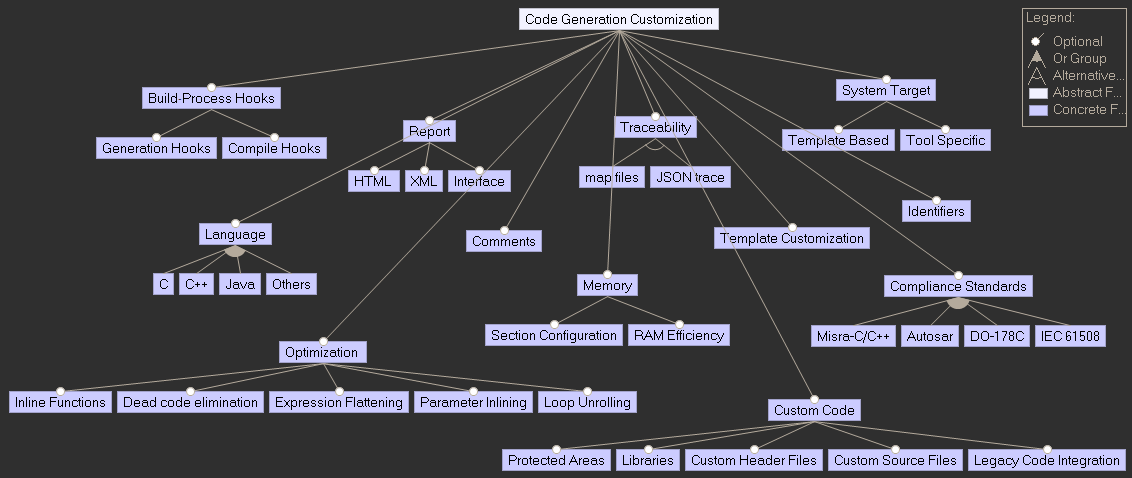
\includegraphics[height=0.4\textwidth]{featureModel.png}
	\caption{Code Gen Config Feature Model}
	\label{fig:feature_model}
\end{figure}

With this, we can have a clearer look at the broader picture. The features suggested are not just the result of analyzing existing code generators like Simulink, OpenModelica, and OpenAPI Generator, they are also derived from a synthesis of industry demands and recurring pain points observed in real-world development environments.

Figure~\ref{fig:feature_model} organizes these configurability aspects into a feature model, grouping them into categories such as Optimization, Traceability, Compliance Standards, Memory Configuration, and Custom Code Integration. The model also highlights optional, alternative, and concrete features that modern code generation tools must support to be competitive and practical across diverse application domains, from automotive (e.g., Autosar, MISRA-C) to safety-critical systems (e.g., DO-178C, IEC 61508).

Additionally, this model also possesses some contrainsts when dealing with certain features, those constraints are the following:

\begin{itemize} 
	\item Misra-C/C++ implies C or C++
	\item Autosar implies C
	\item DO-178C implies C or C++
	\item "IEC 61508" implies C or C++ or Java
	\item "Template Customization" implies "Template Based"
\end{itemize}

This essentially means that most code standards are locked to one or more programming languages, if those programming languages are not selected, the standards does not apply. Similarly, Template Customazation can only be applied to Template Based solutions.

\section{Acceleo and Model-to-Text Transformations} \label{sec:folders_and_files}

To counter the configurability limitations observed in tools like RAMSES, we turn to specialized model-to-text (M2T) transformation technologies. Among these, Acceleo is a highly promising candidate.

\subsection*{Acceleo: An Overview}

Acceleo is an open-source, template-based Eclipse family M2T transformation tool. Its thought model is based on the mapping of formal models (typically in EMF — Eclipse Modeling Framework format) to text artifacts like source code, documentation, or configuration files.

Major benefits of Acceleo are: 
\begin{itemize} 
	\item \textbf{Template-Based Transformation:} Specified templates describe how the elements of a model should be translated into textual form.
	\item \textbf{Strong Eclipse Integration:} Acceleo offers robust integration with the Eclipse IDE, providing instant feedback, syntax coloring, and incremental generation.
	\item \textbf{Structured Code Generation:} Well suited for generating structured, maintainable C/C++ code from high-level models.
\end{itemize}

\begin{tcolorbox}[colback=blue!5, colframe=blue!40!black] Acceleo gives developers the ability to tweak code generation patterns, making the generated codebase more flexible and maintainable. \end{tcolorbox}

\subsection*{Acceleo’s Role in This Thesis}

For this project, Acceleo serves as the basis for enhancing RAMSES' configurability. Through delegating transformation logic to Acceleo templates, we have the aim of: 
\begin{itemize} 
	\item Isolate transformation rules from RAMSES' internal code.
	\item Allow easy extension and modification of code generation patterns.
	\item Facilitate adherence to industrial standards such as MISRA C/C++.
\end{itemize}

This plan promises to transform RAMSES into a more flexible and maintainable toolchain component from one that is rigid code generating.




\section{Existing Work on Configurable Code Generation} \label{sec:configurable_generation}

The search for flexible and customizable code generation is not unique to this thesis. In most domains, tools and techniques have been created to solve the problem of generating high-quality, customizable code from models.

\subsection*{Template-Based Approaches}

Template-based code generation remains the foundation in this field. Some good examples of such tools are \textbf{Acceleo} and \textbf{Simulink templates}: 

\begin{itemize} 
	\item \textbf{Acceleo} allows explicit control of the structure and style of the generated code, making it highly suitable for projects in which compliance with some coding standards or architecture patterns is essential. 
	\item \textbf{Simulink Templates} offers programmers the means to declare patterns of reusable code, with uniform look and feel across several projects and support for custom toolchains and legacy systems.
\end{itemize}

These approaches allow programmers to mold the auto-generated code towards project-specific applications without downgrading underlying models bridging the gap between automated generation and hand-coding, combining efficiency with flexibility.

\subsection*{Hook Functions in TargetLink}

TargetLink, another market leader in code generation tools, comes with the concept of \textbf{hook functions}: pre-compiled points of extension within the generated code that allow developers to plug in their own logic. The facility is most handy in a number of situations. For example, it eases the integration with legacy APIs or platform-dependent libraries and allows developers to add extensions without altering the primary generated code.
\par
In addition, hook functions have the benefit of being customizable without compromising maintainability or upgradability of the generated code. When models evolve, code under it can remain unchanged while introducing custom logic using these extension points. This solution offers a clean trade-off between extending the generated code and offering its long-term maintainability with less effort for future upgrades.

\subsection*{OpenModelica and Multi-Variant Generation}

\textbf{OpenModelica} introduces a higher degree of configurable generation with its support for \textbf{multi-variant code generation}. Through this, engineers are able to:
\begin{itemize} 
	\item Create multiple variants of code based on a common base model.
	\item Tailor outputs for various deployment contexts, hardware configurations, or performance constraints.
\end{itemize}

This variability is completely indispensable in automobile or aircraft production companies, for example, where a single product line might encompass several hardware targets or safety classes.


\subsection*{The Case for Configurability in RAMSES}

Despite its strengths, RAMSES currently has no mechanism for fine-grained extension and configuration.
Specifically:

\begin{itemize} 
	\item Transformation rules are hard-coded, which restricts flexibility.
	\item There is no native support for multi-variant generation or integration points like hook functions. 
\end{itemize}

Including configurability in RAMSES would offer several benefits. It would facilitate the generation of custom code for different deployment environments, making it easier to adapt to specific hardware environments or performance requirements. In addition, the flexibility would simplify maintenance and development of the transformation logic, allowing the tool to better support changing development needs. Finally, by making RAMSES more configurable, it would be easier to interface with industry standards and legacy systems, rendering the tool flexible and applicable in high-speed industries.

\begin{tcolorbox}[colback=green!5, colframe=green!40!black] By adopting template-based generation, RAMSES can evolve into a dynamic, future-proof tool to meet growing embedded system development demands. \end{tcolorbox}

\subsection*{Towards MISRA C/C++ Compliance}

A central element of code generation in configurable code generation, particularly in the field of safety-critical application domains, is to generate \textbf{standard-compliant code}. Strict requirements for safe, portable, and reliable embedded software are presented by the MISRA (Motor Industry Software Reliability Association) C~\cite{Misra_C_2025} and C++~\cite{Misra_Cpp_2023} standards.
\par
Compliance to MISRA plays several principal roles: it enhances software safety by minimizing the likelihood of undefined behavior and runtime errors, guarantees that development processes meet the high standards demanded by industries such as the automobile and aerospace industries where in some instances compliance is mandatory, and is readily compatible with existing toolchains, as most static analysis tools are tailored to enforce MISRA rules.
\par
As we integrate configurable generation facilities into RAMSES, we shall ensure that code generated is MISRA C/C++ compliant.

\begin{tcolorbox}[colback=blue!5, colframe=blue!40!black] Flexible code generators need to not just conform to project requirements but also apply vital industry standards such as MISRA to guarantee safety and reliability. \end{tcolorbox}




 %
% Please note that
% \begin{center}
%   \textbf{\large this package and template are not official for FCT/NOVA}.
% \end{center}



% \printbibliography[heading=subbibliography, segment=\therefsegment, title={\bibname\ for chapter~\thechapter}]
